
\subsection{BoT-IoT}

\subsubsection{Descripción}

BoT-IoT es un dataset creado por la University of New South Wales Canberra, Australia \cite{DBLP:journals/corr/abs-1811-00701}. Para generarlo, se desarrolló un entorno de red realista, consistiendo en plataformas de red, dispositivos IoT simulados y extracción de características y análisis forense. Para generar el tráfico benigno, se hace uso de la herramienta Ostinato \cite{ostinato} y para la extracción de características a partir de los flujos de red se hace uso de Argus \cite{argustool} y a continuación es enriquecido con información de los flujos concurrentes. Los sensores simulados publican mensajes por MQTT y consisten en una estación meteorológica (la cual genera información de la presión del aire, humedad y temperatura) una nevera inteligente (la cual genera información de temperatura y la ajusta según unos límites), luces activadas por movimiento (las cuales se apagan y se encienden según una señal generada pseudoaleatoriamente), una puerta de un garaje (la cual se abre y se cierra según una entrada probabilística) y un termostato inteligente (el cual regula la temperatura activando un sistema de aire acondicionado).

La red interna dispone de unos elementos de la red interna que consisten en 10 máquinas virtuales, tres máquinas adicionales en un clúster VMWare y un router:

\begin{itemize}
    \item Cuatro máquinas virtuales con Kali Linux como atacantes (192.\-168.\-100.\-147 a 192.\-168.\-100.\-150).
    \item Máquina virtual con Ubuntu Server (192.168.100.3), el cual ofrece diversos servicios (DNS, email, FTP, HTTP y SSH), además de servicios IoT simulados.
    \item Máquina virtual con Ubuntu Mobile (192.168.100.5).
    \item Máquina virtual con Windows 7 (192.168.100.6).
    \item Máquina virtual con Metasplotaible (192.168.100.7), una distribución específicamente diseñada para ser vulnerable contra la cual hacer pruebas.
    \item Máquina virtual para hacer la captura de tráfico (192.168.100.4).
    \item Router pfSense (192.168.1.100.1)
    \item Tres máquinas en un clúster VMWare (192.168.1.100.(20, 22, 24)).
\end{itemize}

En el dataset se han generado ataques mediante nmap, hping3, xprobe2, golden-eye y Metasploit. Según el paper, tenemos 3 tipos principales: 
\begin{enumerate}
    \item \textbf{Recolección de información} (Reconnaissance): ataques en los cuales se trata de obtener información sobre potenciales víctimas a través de escanear los sistemas. Hay dos subcategorías de ataques realizados:
    \begin{enumerate}
        \item \textbf{Escaneo de puertos}(Service\_Scan): se realizan peticiones hacia diferentes puertos y, en caso de recibir respuesta, se puede saber que el sistema está escuchando en este. En caso de ser un puerto en el cual se suele ofrecer un servicio, se puede suponer que este se encuentra disponible.
        \item \textbf{Detección de huellas digitales de los sistemas} (OS\_Fingerprint): a partir de hacer peticiones y/o tráfico capturado y comparando con ejemplos preexistentes, se pueden llegar a identificar el sistema operativo en uso.
    \end{enumerate}
    \item \textbf{Denegación de servicio}: ataques que tratan de provocar que un servicio deje de estar disponible a usuarios legítimos. Este puede ser distribuido (DDoS) o no (DoS). Normalmente, estos ataques tratan de abusar el funcionamiento de un protocolo para provocar que se reduzca la CPU, la RAM o el ancho de banda disponible de manera drástica en el hardware ofreciendo un servicio. Las subcategorías de ataques en este caso consisten en los tres protocolos utilizados: TCP, UDP y HTTP.
    \item \textbf{Robo de información} (Theft): ataques en los que se trata de comprometer la seguridad de un sistema para la obtención de información sensible. Se definen dos subcategorías:
    \begin{enumerate}
        \item \textbf{Robo de datos}(Data\_Exfiltration): Se obtiene acceso no autorizado a ficheros del sistema, los cuales se descargan a la máquina atacante.
        \item \textbf{Captura de teclas} (Keylogging): Se obtienen privilegios elevados en un sistema, con los cuales se utilizan para leer las pulsaciones entradas en un sistema y enviar los registros a la máquina atacante.
    \end{enumerate}
\end{enumerate}


\subsubsection{Contenidos CSVs}

El conjunto de datos procesados está separado en diferentes grupos. Por un lado, tenemos todos los flujos con sus características y etiquetados. Estos se encuentran en carpeta llamada 'Entire Dataset', separados por incrementos de unos 220 MiB y en otra llamada "Ground Truth" separados por  el ataque que se encontraba activo en cada momento. Por otro lado, tenemos un muestreo del 5\%, el cual tiene algunos archivos CSV de flujos con características adicionales y otro con características seleccionadas. Adicionalmente, hay dos archivos adicionales basados en este último como división de entrenamiento y de test. Los scripts utilizados para la extracción y representación de los datos son \texttt{extract\_info\_botiot\_csvs\_full\_dataset.py} y \texttt{plot\_info\_botiot\_csvs.py} disponibles en TODO DEFINIR.

No hay ningún tipo de solapación en los archivos 'Ground Truth', los flujos etiquetados en cada uno consisten en flujos benignos y los ataques específicos. En la figura \ref{fig:botiot_results} podemos ver cómo los flujos consisten principalmente en ataques DoS y DDoS sobre TCP y UDP y de recolección de información. El tráfico Benigno, como podemos ver en este caso, también se encuentra infrarepresentado respecto al total, cosa que puede ser que no corresponda con un tráfico normal. 

Si observamos la línea temporal de la figura \ref{fig:botiot_timeline}, podemos ver cómo las diferentes categorías de ataques están repartidas en el tiempo de manera distinta. En el caso de los ataques de recolección de información, el análisis de los servicios se extiende durante unos seis días y de detección del sistema operativo durante uno y medio. Para los casos de denegación de servicio, cada subcategoría dura alrededor de una hora. Finalmente, para los ataques de robo de información tienen una duración limitada. Las cantidades de tráfico visto y sus extensiones temporales son consistentes con la tipología de ataque. El escaneo se realiza durante mucho tiempo para tratar de pasar desapercibido. En la denegación se genera mucho volumen de tráfico en poco tiempo. Finalmente, en el robo de información se ejecuta el proceso de ataque específico en el menor tiempo y cantidad de tráfico posible.

\begin{figure}[H]
    \begin{center}
        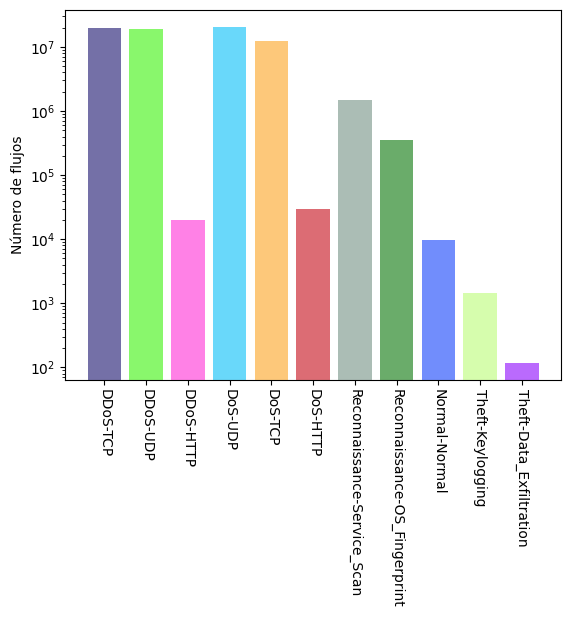
\includegraphics[width=0.49\linewidth]{media/botiot_csv_day_results.png}
    \end{center}
    \captionsetup{justification=centering}
    \caption{Línea temporal de las trazas con categorias (debajo) y subcategorias (arriba)}\label{fig:botiot_results}
\end{figure}

\begin{figure}[!htb]
    \begin{center}
        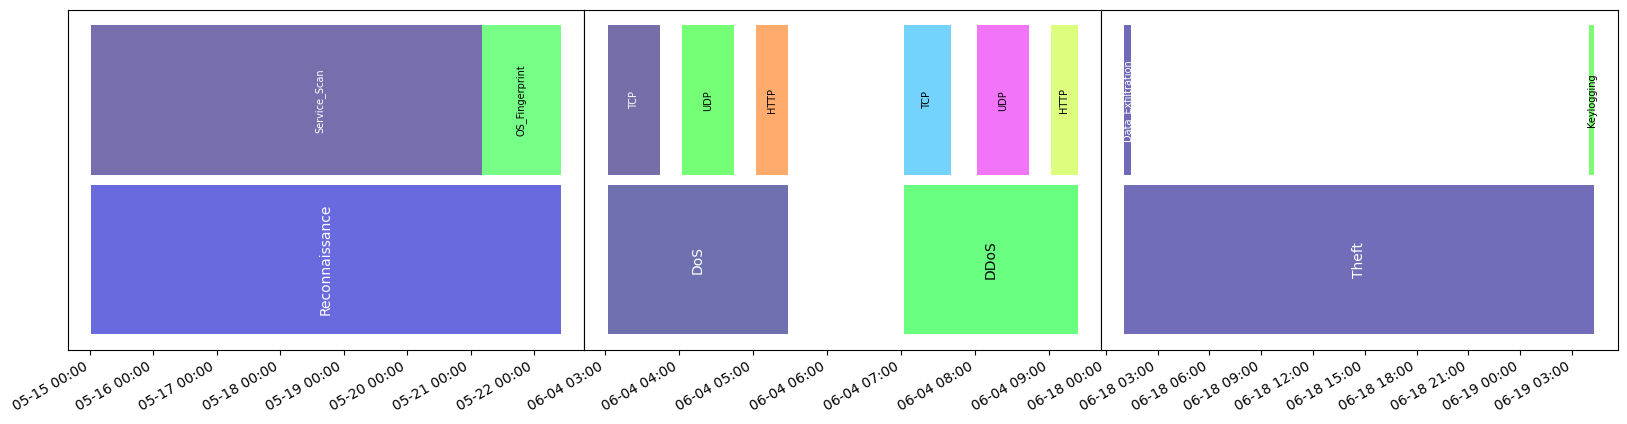
\includegraphics[width=1\linewidth]{media/botiot_csv_timeline.png}
    \end{center}
    \captionsetup{justification=centering}
    \caption{Línea temporal de las trazas con categorias (debajo) y subcategorias (arriba)}\label{fig:botiot_timeline}
\end{figure}

En total, hay 46 características disponibles en el dataset y explicadas en una tabla tanto en el paper original como en el conjunto de datos descargables. Manteniendo la capitalización de la tabla dentro del conjunto de datos, las características consisten en:

\begin{enumerate}
    \item \textbf{pkSeqID}: Identificador de fila
    \item \textbf{Stime}: Tiempo de inicio del flujo expresado en tiempo Unix. La representación concreta es un número decimal donde la parte entera es los segundos.
    \item \textbf{Flgs}: Indicador de estado de flujo. Es una expresión textual, el formato, el cual se puede ver en el manual de ra \cite{ratool}
    \item \textbf{flgs\_number}: Representación de 'Flgs' en formato numérico. No aparece en 'Entire Dataset', tan solo en la versión reducida al 5\%.
    \item \textbf{Proto}: Representacion textual del protocolo the mayor nivel utilizado
    \item \textbf{proto\_number}: Representación numérica de 'Proto'. No parece utilizar el de RFC-1700 \cite{rfc1700}, ya que TCP le asigna un 1 en vez de un 6. Adicionalmente, no aparece en 'Entire Dataset', tan solo en la versión reducida al 5\%.
    \item \textbf{Saddr}: Dirección IP de origen.
    \item \textbf{Sport}: Puerto IP de origen.
    \item \textbf{Daddr}: Dirección IP de destino.
    \item \textbf{Dport}: Puerto IP de destino.
    \item \textbf{Pkts}: Número de paquetes enviados en ambos sentidos
    \item \textbf{Bytes}: Número de bytes enviados en ambos sentidos
    \item \textbf{State}: Último estado de la conexión expresado en forma textual.
    \item \textbf{state\_number}: Representación de 'State' en formato numérico. No aparece en 'Entire Dataset', tan solo en la versión reducida al 5\%.
    \item \textbf{Ltime}: Tiempo de finalización del flujo expresado en tiempo Unix. La representación concreta es un número decimal donde la parte entera es los segundos.
    \item \textbf{Seq}: Número de secuencia de Argus.
    \item \textbf{Dur}: Duración total, expresado en segundos,
    \item \textbf{Mean}: Duración media de los registros agregados en el momento.
    \item \textbf{Stddev}: Desviación estándar de la duración de los registros agregados en el momento.
    \item \textbf{Sum}: Suma de la duración de los registros agregados en el momento.
    \item \textbf{Min}: Duración mínima de los registros agregados en el momento.
    \item \textbf{Max}: Duración máxima de los registros agregados en el momento.
    \item \textbf{Spkts}: Número de paquetes enviados hacia el emisor inicial
    \item \textbf{Dpkts}: Número de paquetes enviados hacia el destino inicial
    \item \textbf{Sbytes}: Número de bytes enviados hacia el emisor inicial
    \item \textbf{Dbytes}: Número de bytes enviados hacia el destino inicial
    \item \textbf{Rate}: Cadencia total de paquetes en ambos sentidos
    \item \textbf{Srate}: Cadencia de paquetes hacia el emisor inicial
    \item \textbf{Drate}: Cadencia de paquetes hacia el destino inicial
    \item \textbf{TnBPSrcIP}: Número total de bytes hacia la dirección IP del emisor inicial en la ventana del momento. Solo aparece en la versión reducida al 5\%.
    \item \textbf{TnBPDstIP}: Número total de bytes hacia la dirección IP del destino inicial en la ventana del momento. Solo aparece en la versión reducida al 5\%.
    \item \textbf{TnP\_PSrcIP}: Número total de paquetes hacia la dirección IP del emisor inicial en la ventana del momento. Solo aparece en la versión reducida al 5\%.
    \item \textbf{TnP\_PDstIP}: Número total de paquetes hacia la dirección IP del destino inicial en la ventana del momento. Solo aparece en la versión reducida al 5\%.
    \item \textbf{TnP\_PerProto}: Número total de paquetes del protocolo en la ventana del momento. Solo aparece en la versión reducida al 5\%.
    \item \textbf{TnP\_Per\_Dport}: Número total de paquetes hacia el puerto de destino inicial en la ventana del momento. Solo aparece en la versión reducida al 5\%.
    \item \textbf{AR\_P\_Proto\_P\_SrcIP}: Cadencia media del protocolo y dirección IP del emisor inicial en la ventana del momento. Solo aparece en la versión reducida al 5\%.
    \item \textbf{AR\_P\_Proto\_P\_DstIP}: Cadencia media del protocolo y dirección IP del destino inicial en la ventana del momento. Solo aparece en la versión reducida al 5\%.
    \item \textbf{N\_IN\_Conn\_P\_SrcIP}: Número de conexiones entrantes por IP del emisor inicial. Solo aparece en la version reducida al 5\%.
    \item \textbf{N\_IN\_Conn\_P\_DstIP}: Número de conexiones entrantes por IP del destino inicial. Solo aparece en la version reducida al 5\%.
    \item \textbf{AR\_P\_Proto\_P\_Sport}: Cadencia media del protocolo y puerto  de origen inicial en la ventana del momento. Solo aparece en la versión reducida al 5\%.
    \item \textbf{AR\_P\_Proto\_P\_Dport}: Cadencia media del protocolo y puerto  de destino inicial en la ventana del momento. Solo aparece en la versión reducida al 5\%.
    \item \textbf{Pkts\_P\_State\_P\_Protocol\_P\_DestIP}: Número de paquetes del estado del flujo, protocolo y dirección IP de destino inicial en la ventana del momento. Solo aparece en la version reducida al 5\%.
    \item \textbf{Pkts\_P\_State\_P\_Protocol\_P\_SrcIP}: Número de paquetes del estado del flujo, protocolo y dirección IP de origen inicial en la ventana del momento. Solo aparece en la versión reducida al 5\%.
    \item \textbf{Attack}: Indicador de flujo de ataque. Se utiliza 0 para tráfico benigno y 1 para tráfico maligno.
    \item \textbf{Category}: Categoría del ataque o "Normal" si es benigno.
    \item \textbf{Subcategory}: Subcategoría del ataque o "Normal" si es benigno.
\end{enumerate}


\subsubsection{Contenidos PCAPs}

El dataset BoT-IoT ofrece 344 archivos (69.4 GiB) de trazas de red por cada categoría y subcategoría de ataque realizado. Tenemos, por cada categoría, 48 archivos (9.7 GiB) de los ataques de recolección de información, 130 (25.9 GiB) para la denegación de servicio no distribuida, 150 (30.2 GiB) para la denegación de servicio distribuida y 16 (3.5 GiB) para el robo de información. Los archivos se encuentran divididos en carpetas según su categoría y su subcategoría. Los scripts utilizados para la extracción de datos es \texttt{extract\_info\_botiot\_pcaps\_tshark.sh} y el utilizado para la representacion de estos es \texttt{evaluate\_info\_botiot\_pcaps\_tshark.py} disponibles en TODO DEFINIR.

En los PCAP, aparecen direcciones IP diferentes del testbed (192.168.1.100.0/24) de las mencionadas en el paper original. Concretamente, podemos ver que aparecen adicionalmente 192.168.100.27, 192.168.100.46 y 192.168.100.55, además de la dirección de broadcast 192.168.100.255. Por otro lado, no se han detectado tráfico hacia o desde las máquinas del clúster VMWare con direcciones IP 192.168.1.100.(20, 22, 24). Respecto al número de direcciones IP únicas, podemos observar que aparecen 293 de estas, menos que en CICDDos2019.


Para este dataset, también se han generado histogramas con la distribución de la duración de los flujos, número de tramas y número de bytes para poder compararlos con los futuros resultados de la herramienta y comprobar que son consistentes. Si observamos la figura \ref{fig:botiot_pcap_duration_distribution}, podemos notar que en este caso también hay muchos flujos los cuales su duración es relativamente corta y luego cierta variedad de flujos de mayor duración, siendo esta menor y pareciendo que hay ciertas agrupaciones. Si miramos la distribución del número de tramas, podemos ver en la figura \ref{fig:botiot_pcap_frames_distribution} que hay dos picos bajo 100 tramas y luego una agrupación más ancha entre 5 000 y  50 000 y otro pico entre 100 000 y 1 000 000. Respecto los bytes, podemos ver en la figura \ref{fig:botiot_pcap_bytes_distribution} que la situación es diferente. La cantidad de bytes en diferentes flujos, pese a que en algunos puntos haya valles, parece estar más repartida.


\begin{figure}[H]
    \begin{center}
        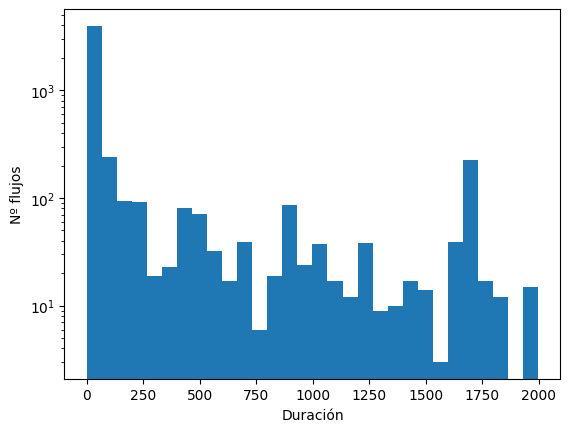
\includegraphics[width=0.40\linewidth]{media/botiot_pcap_duration_distribution.png}
    \end{center}
    \captionsetup{justification=centering}
    \caption{Distribución duraciones de flujos en BoT-IoT}\label{fig:botiot_pcap_duration_distribution}
\end{figure}

\begin{figure}[H]
    \minipage{0.49\textwidth}
      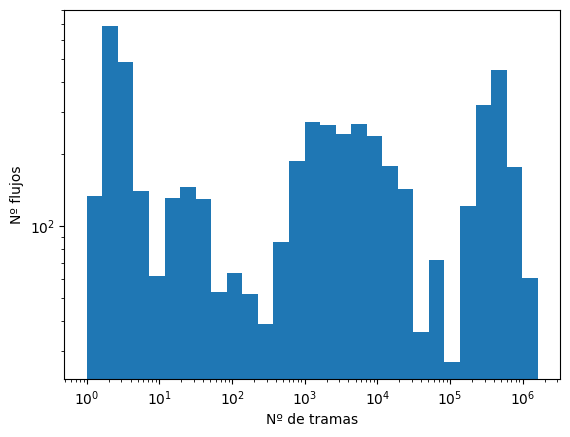
\includegraphics[width=\linewidth]{media/botiot_pcap_frames_distribution.png}
      \captionsetup{justification=centering}
      \caption{Distribución número de tramas en flujos en BoT-IoT}\label{fig:botiot_pcap_frames_distribution}
    \endminipage\hfill
    \minipage{0.49\textwidth}
      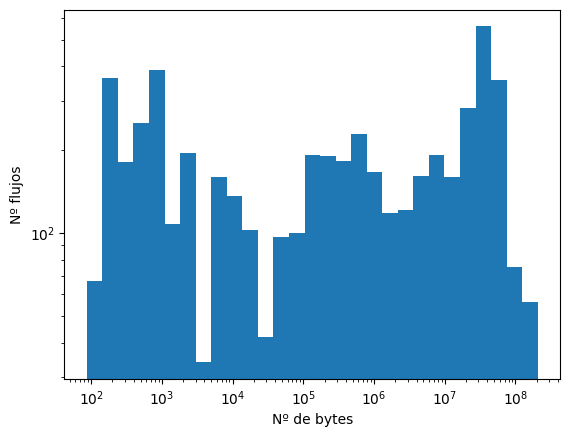
\includegraphics[width=\linewidth]{media/botiot_pcap_bytes_distribution.png}
      \captionsetup{justification=centering}
      \caption{Distribución número de bytes en flujos en BoT-IoT}\label{fig:botiot_pcap_bytes_distribution}
    \endminipage\hfill
\end{figure}

En la tabla \ref{table:botiotprotocolsip} podemos ver el resultado del análisis con tshark sobre la repartición de los diferentes protocolos de transporte sobre IPv4. Como podemos ver, nos indica que la mayoría (68.549\%) de los datos van sobre UDP y el resto se encuentra principalmente contenido en TCP (31.450\%). Hay tramas que no se han podido identificar, pero es una cantidad marginal (0.001\%). A diferencia de CICDDos2019, no tenemos otros protocolos residuales.

%Generated with /workspaces/tfg/scripts/evaluate_info_botiot_tshark.py
\begin{table}[H]
    \begin{center}
        \begin{tabular}{|c | c c|} 
            \hline
            \textbf{Protocolo} & \textbf{Nº Tramas} & \textbf{Porcentaje}\\
            \hline\hline
IP & 5.50e+08 & 100.000 \\
UDP & 3.77e+08 & 68.549 \\
TCP & 1.73e+08 & 31.450 \\
NONE & 3.98e+03 & 0.001 \\
            \hline
        \end{tabular}
    \end{center}
    \caption{Protocolos identificados analizando exclusivamente la capa IP en BoT-IoT}
    \label{table:botiotprotocolsip}
\end{table}


Si miramos la cantidad de información transmitida por las diferentes capas de red y de transporte en la tabla \ref{table:botiotprotocols}, podemos ver cómo la mayor parte del tráfico sigue consistiendo en UDP y TCP, teniendo algo de tráfico residual en ICMP, IGMP y no identificado (data). De los 64.2 GiB presentes, menos de 4 MiB no consisten en tráfico IPv4. En términos de bytes, UDP y TCP comprenden una cantidad similar (28.6 GiB y 32.5 GiB, respectivamente) a pesar de que haya casi el doble de tramas que utilizan UDP respecto TCP. De la misma manera que en CICDDos2019, los protocolos residuales detectados en la capa de transporte sobre IP son diferentes a los de la tabla \ref{table:botiotprotocolsip}.

%Generated with /workspaces/tfg/scripts/evaluate_info_botiot_tshark.py
\begin{table}[H]
    \begin{center}
        \begin{tabular}{|c c c | c c c|} 
            \hline
            \textbf{L0} & \textbf{L1} & \textbf{L2} & \textbf{Tramas} & \textbf{Bytes} & \textbf{Nº subprotocolos}\\
            \hline\hline
eth &- &- & 5.50e+08 & 61.2GiB & 3 \\
eth &ip &- & 5.50e+08 & 61.2GiB & 5 \\
eth &ip &udp & 3.76e+08 & 28.6GiB & 22 \\
eth &ip &tcp & 1.73e+08 & 32.5GiB & 34 \\
eth &ip &icmp & 6.70e+05 & 45.1MiB & 18 \\
eth &ip &data & 1.00e+01 & 14.8KiB & 0 \\
eth &ip &igmp & 1.80e+01 & 1.1KiB & 0 \\
eth &arp &- & 6.00e+04 & 3.4MiB & 0 \\
eth &ipv6 &- & 1.95e+02 & 20.8KiB & 2 \\
eth &ipv6 &icmpv6 & 9.50e+01 & 6.5KiB & 0 \\
eth &ipv6 &udp & 1.00e+02 & 14.3KiB & 2 \\
            \hline
        \end{tabular}
    \end{center}
    \caption{Primeras tres capas de protocolos identificados en BoT-IoT}
    \label{table:botiotprotocols}
\end{table}


Finalmente, si abrimos cualquier traza de red, podemos observar que solo se utiliza 'Ethernet II' para la capa de enlace, como podemos ver en la figura \ref{fig:botiot_pcap_ethii_packet}. Cabe notar que en algún caso aparecen paquetes marcados con una alerta, como en la figura \ref{fig:botiot_pcap_ethii_packet_warn}, indicando que el origen de la trama no debería contener una dirección de grupo.

\begin{figure}[H]
    \minipage{0.49\textwidth}
      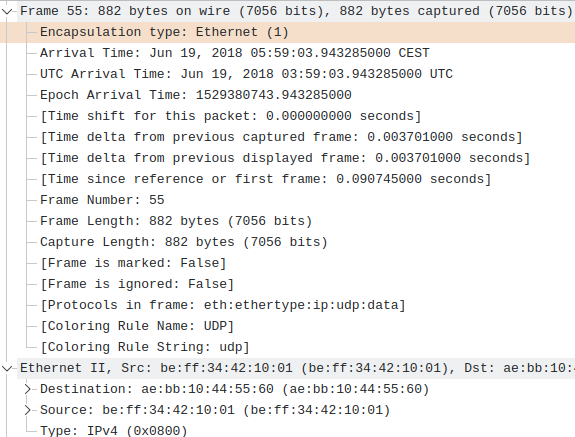
\includegraphics[width=\linewidth]{media/botiot_pcap_ethii_packet.png}
      \captionsetup{justification=centering}
      \caption{Paquete sin alerta en BoT-IoT}\label{fig:botiot_pcap_ethii_packet}
    \endminipage\hfill
    \minipage{0.49\textwidth}
      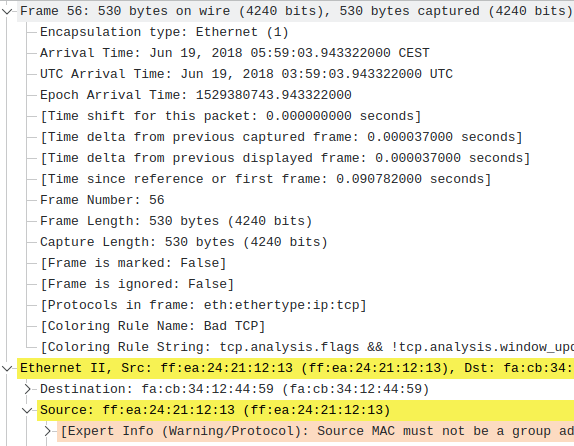
\includegraphics[width=\linewidth]{media/botiot_pcap_ethii_packet_warn.png}
      \captionsetup{justification=centering}
      \caption{Paquete con alerta BoT-IoT}\label{fig:botiot_pcap_ethii_packet_warn}
    \endminipage\hfill
\end{figure}
